\chapter{Guida all'utente}
\section{Avvio dell'applicazine}
\noindent Per poter utilizzare l'applicativo in maniera corretta bisogna
\begin{enumerate}
    \item Avviare il processo server "\texttt{StartServer}";
    \item Avviare il processo client "\texttt{StartApplication}".
\end{enumerate}

\section{Accesso}
\noindent Per assegnare il ruolo di "Amministratore" a un utente, è necessario effettuare l'inserimento direttamente nel database per garantire un adeguato controllo dei privilegi e una buona gestione degli accessi.\\
\\
Per utilizzare l'applicazione, sia il cliente che l'amministratore (agente immobiliare) devono effettuare l'accesso. Tale procedura richiede l'inserimento di un nome utente e di una password.\\
Al momento del tentativo di accesso, il sistema, tramite il \texttt{Main Handler} interroga il database per verificare se l'utente è registrato e se le credenziali inserite sono corrette.\\

\begin{figure}[h]
\begin{tabular}{ll}
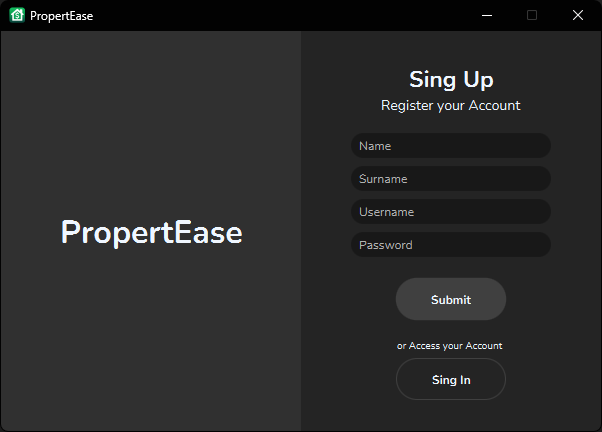
\includegraphics[scale=0.35]{signup.png}
&
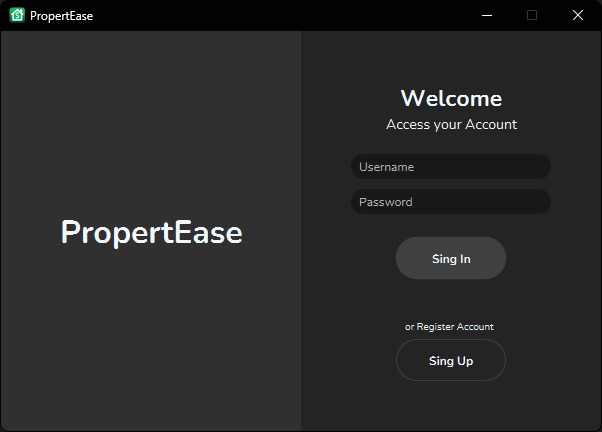
\includegraphics[scale=0.35]{login.png}
\end{tabular}
\caption{(sx): registrazione (dx): accesso}
\label{Fig:Race}
\end{figure}

\noindent Nel caso in cui un utente non risulti registrato, è possibile effettuare la registrazione tramite la sezione dedicata denominata "Sign Up". In questa sezione, vengono richiesti il nome, il cognome, il nome utente e la password.\\
\textit{N.B.:} Sono implementati controlli sull'unicità del nome utente. Se i dati inseriti sono corretti, le credenziali vengono memorizzate nel database.
\section{Utilizzo applicazione}
\subsection{Utente}
\noindent L'interfaccia utente post-login è molto intuitiva, con le card cliccabili per ogni immobile ed un tab sulla sinistra con i suoi appuntamenti.\\
\\
Cliccando su una della card, si è reindirizzati alla pagina in cui sono mostrati i dettagli degli immobili e dove  è possibile prenotare un appuntamento.\\
\\
La navbar in alto permette la navigazione delle pagine.

\begin{figure}[htbp]
    \centering
    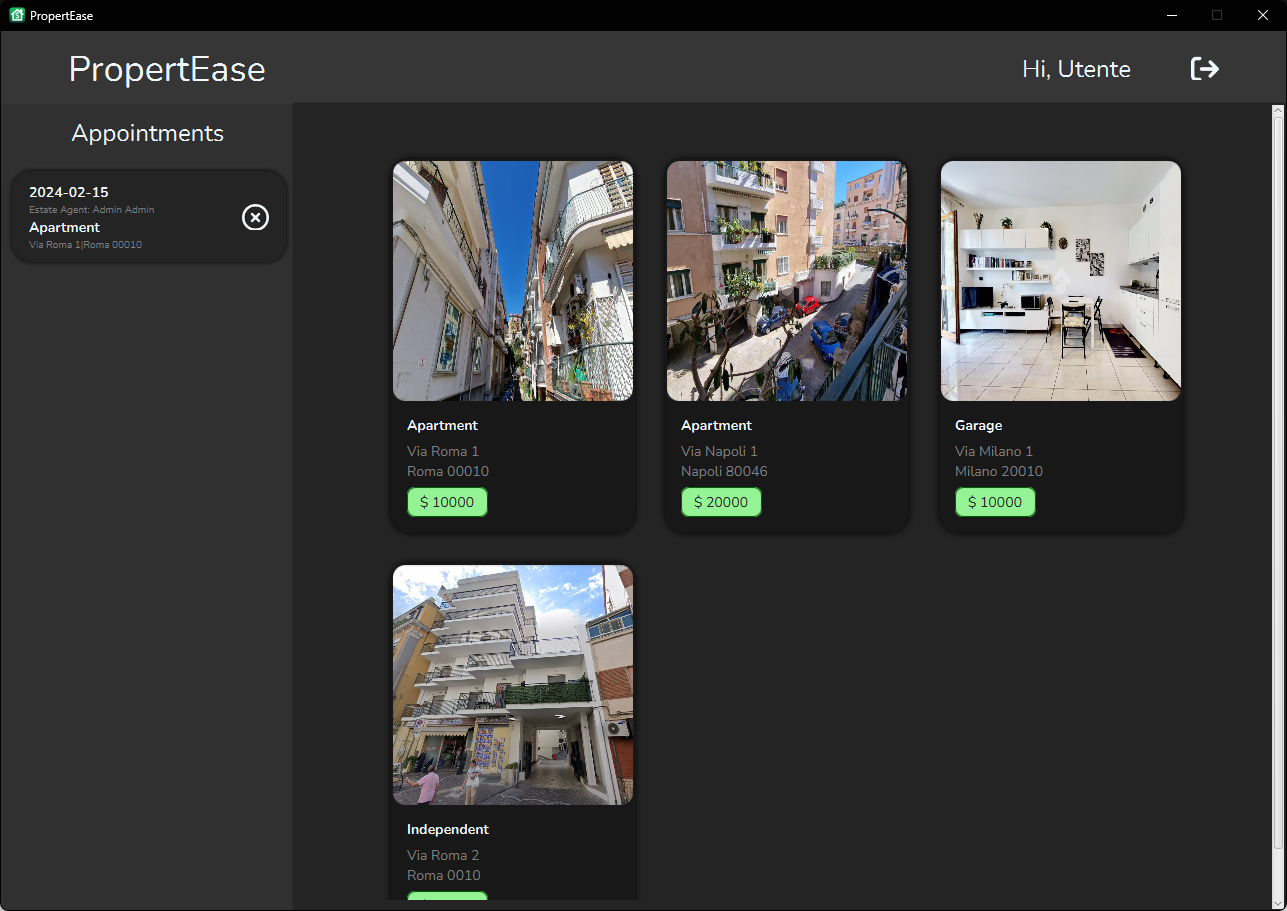
\includegraphics[width=\textwidth,height=\textheight,keepaspectratio]{mainDashboard.png}
    \caption{Schermata principale dell'applicazione}
\end{figure}
\begin{figure}[htbp]
    \centering
    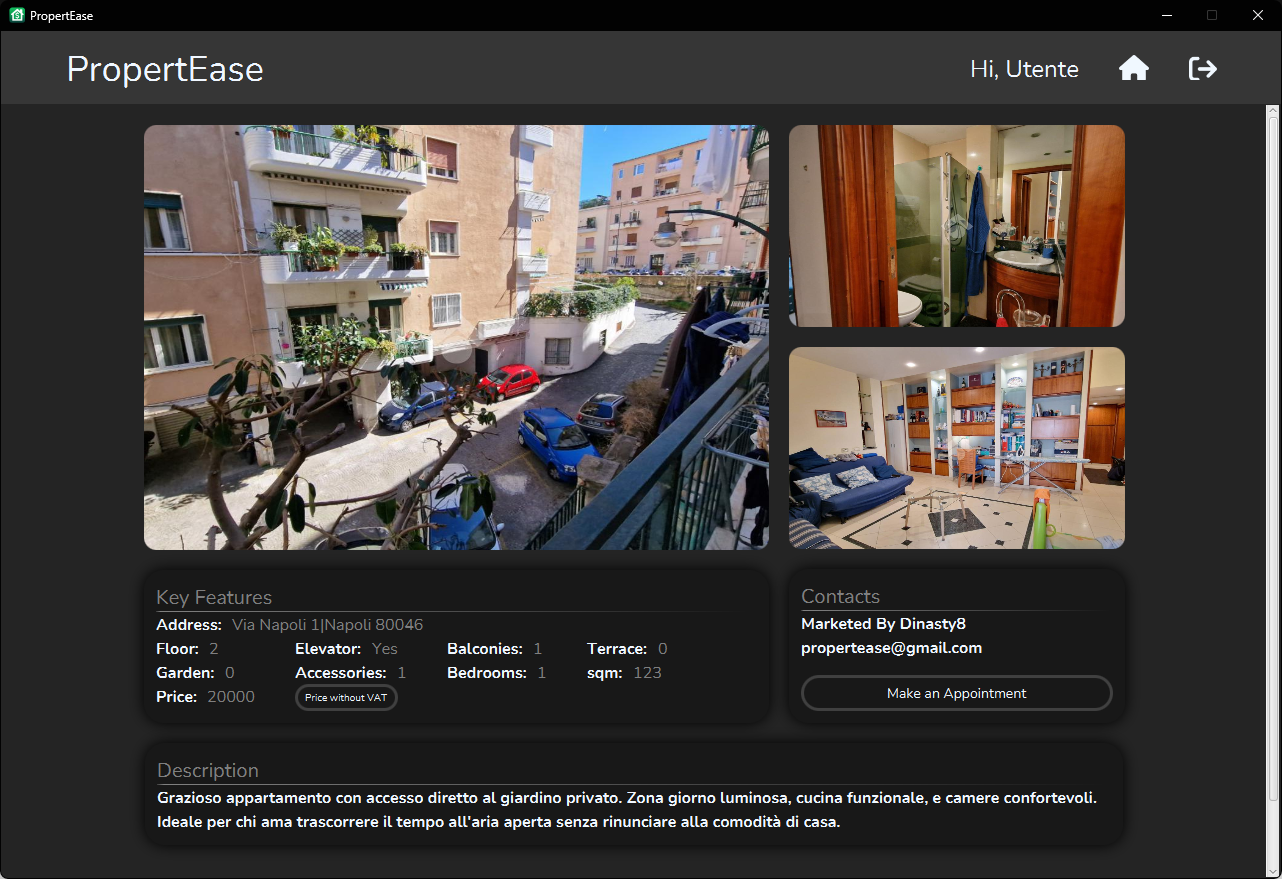
\includegraphics[width=\textwidth,height=\textheight,keepaspectratio]{houseView.png}
    \caption{Schermata dei dettagli di un immobile}
\end{figure}

\subsection{Amministratore}
\noindent Oltre a quanto sopracitato per l'utente, l'amministratore avrà le varie funzioni sempre in pulsanti locati in alto a destra della GUI.\\
Tramite questi bottoni, egli potrà inserire, rimuovere e aggiornare gli immobili del database.\\

\subsection{Errori}
\noindent per ogni operazione di modifica, inserimento ed eliminazione su database, è stato inserito, dal punto di vista di interfaccia, un pop-up di conferma o metodi di ripristino dei dati.

\begin{figure}[h]
\begin{tabular}{ll}
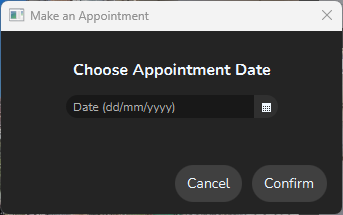
\includegraphics[scale=0.65]{takeAppointment.png}
&
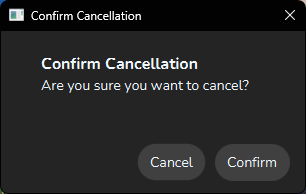
\includegraphics[scale=1]{confirmCancellation.png}
\end{tabular}
\caption{conferma di presa (sx) e cancellazione (dx) di un appuntamento}
\label{Fig:Race}
\end{figure}